\section{Experimental results}
\label{section:results} We have implemented the algorithms with
multi-threading support from C++ 11, and conducted the experiments on
Linux PCs with Intel Core i7 4790 processor with 4 cores. We have used
the Graph-cuts optimization code written by Veksler, using the libraries
provided by Boykov and
Kolmogorov~\cite{middlebury_mrf,alpha_expansion,what_energy_can_be_min_by_gc,mrf_experimental}.
% [2] Fast Approximate Energy Minimization via Graph Cuts.
%         Y. Boykov, O. Veksler, and R. Zabih.
%         In IEEE Transactions on Pattern Analysis and Machine Intelligence
%         (PAMI), vol. 23, no. 11, pages 1222-1239, November 2001.  
%
%     [3] What Energy Functions can be Minimized via Graph Cuts?
%         V. Kolmogorov and R. Zabih. 
%         In IEEE Transactions on Pattern Analysis and Machine Intelligence
%         (PAMI), vol. 26, no. 2, pages 147-159, February 2004. 
%         An earlier version appeared in European Conference on Computer
%         Vision (ECCV), May 2002.
%
%     [4] An Experimental Comparison of Min-Cut/Max-Flow Algorithms for
%         Energy Minimization in Vision. 
%         Y. Boykov and Vladimir Kolmogorov.
%         In IEEE Transactions on Pattern Analysis and Machine Intelligence
%         (PAMI), vol. 26, no. 9, pages 1124-1137, September 2004. 
We have used the QPBO and TRW-S implementations by
Kolmogorov~\cite{QPBO, TRW-S_implementation}. We now look at our
experimental results for the three problems.



% To evaluate the effectness of different parallel structures, we plot
% the energy minimization process against time. We define the energy of
% a parallel optimization system at a certain time as the minimum energy
% of all threads at that time.

\mysubsubsection{Stereo}

\noindent We have chosen 7 images with the resolution of $695\times555$
from the Book sequence of Middlebury stereo dataset for our
experiment~\cite{middlebury_stereo}. The number of disparity labels is
set to 256.
%
Since the order of labels is important for the expansion techniques,
we have used the same random order for all algorithms to avoid any
bias.
%
% In PAE, SF-MF, SF-SS and SF algorithms, the proposal generator in each
% thread can only generate constant-label proposals within a evenly split
% subset of all labels.



Fig.~\ref{fig:stereo_global} compares the converegence rate of the
competing methods. Note that we define the energy of a multi-threading
system to be the energy of the best solution found so far.
%
\begin{figure}[tb]
  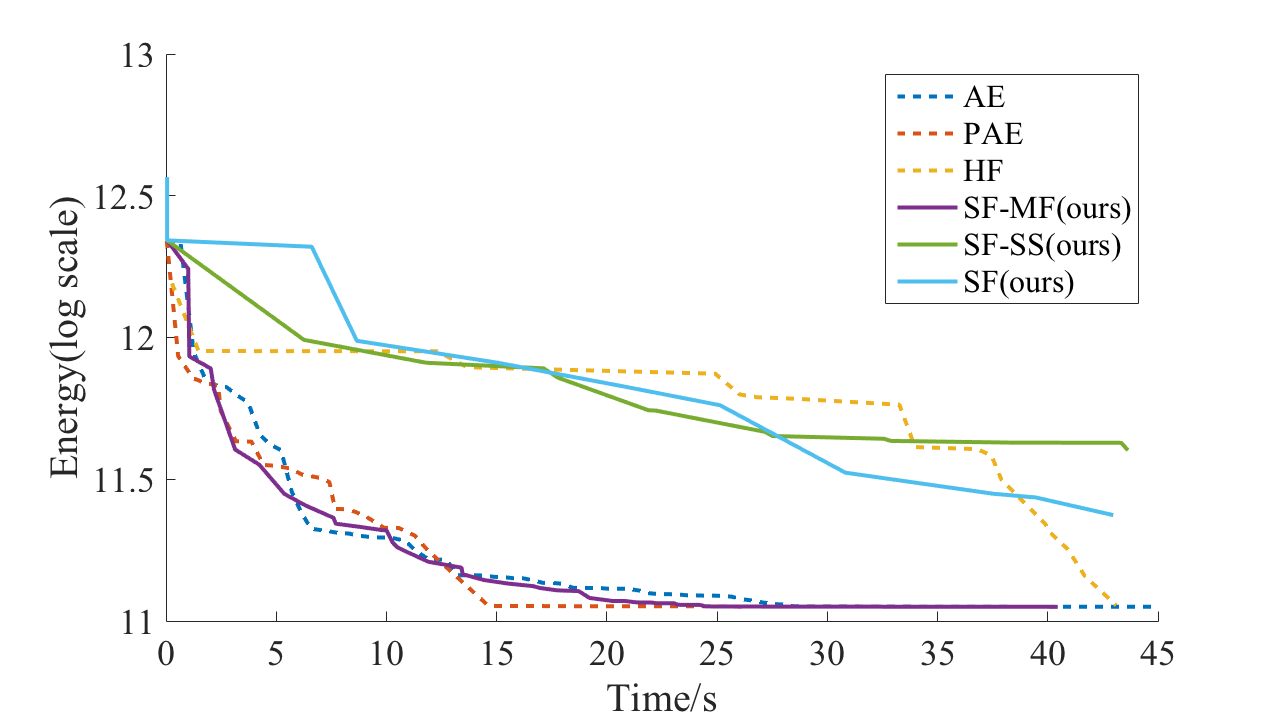
\includegraphics[width=\columnwidth]{figure/stereo_global.png}
 \caption{Energy plots for the stereo problem. The energy is in the log
 scale. For a multi-threading algorithm, the energy at a given moment is
 defined to be the best solution so far.} \label{fig:stereo_global}
\end{figure}
%
One unusual outcome is that Sequential Alpha Expansion and Parallel
Alpha Expansion (PAE) have the same convergence speed, indicating that
the stereo problem is a very easy one.
%This is well known in a community and this fact was rather expected.
Our approaches with multi-way fusion (SF-SS or SF) are the slowest kind,
because the TRW-S for multi-way fusion is slower than multiple Alpha
Expansion steps, and this stereo problem is too easy to gain benefits
through mulit-way fusion.
%
%Another interesting observation is that the Hierarchical Fusion can
%achieve good energy only when they merge solutions at the top of the
%tree.
%
%  both PAE and SF-MF converge faster
% than sequential method. However, since fusing solutions with multiple
% labels by QPBO is slower than a single $\alpha$-expansion, PAE method
%
% Finally, the line of hierarchy fusion only makes
% jump when fusing on root node of the tree. This is because any fusion
% step on non-root nodes only have partial label information.
%We recoreded both single thread energy and system energy against
%time.
%
Fig. \ref{fig:stereo_threads} shows the energy plot per thread
for SF-MF (ours) and PAE. The graph for PAE again confirms that the
stereo is an easy problem, because all the threads are quickly
converging to a solution before the final sequential fusion.
%shows the per-thread energy
%minimization process in SF-MF and PAE. The per-thread energy in SF-MF
%architecture decreases more uniformly than that of PAE. In the
%scenario where we need to query the best solution so far before the
%whole optimization converges, SF-MF architecture is a better choice.
\begin{figure}[tb]
  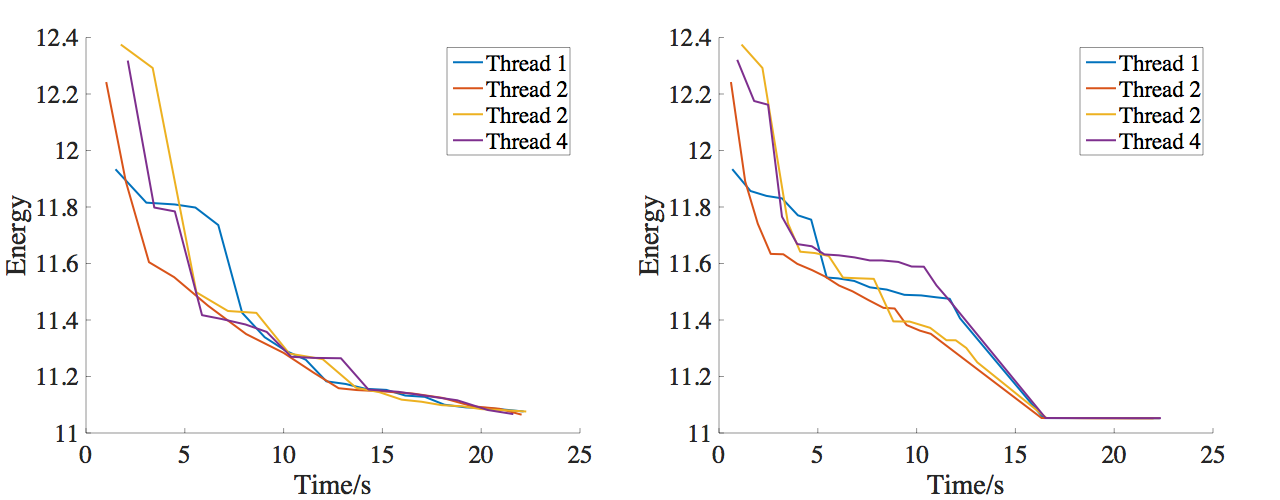
\includegraphics[width=\columnwidth]{figure/stereo_threads.png}
  \caption{Energy plots per thread for the stereo proble for SF-MF (left) and
 Parallel Alpha Expansion (right).
} \label{fig:stereo_threads}
\end{figure}

For an easy optimization problem such as stereo with strong unary terms
and submodular pairwise terms, our full architecture with solution
sharing and multiway fusion actually makes convergence slower due to the
overhead of fusion and multi-threading.




% over-sophisticated fusion algorihtm and multi-threading
% overhead. However, we can easily configure the architecture to make it
% better fit the problem, e.g. turn off multiway fusion and/or solution
% sharing.





% We define the energy of
% a parallel optimization system at a certain time as the minimum energy
% of all threads at that time.

\mysubsubsection{Optical Flow}


% \hang{figure file missing}
\begin{figure}[tb]
  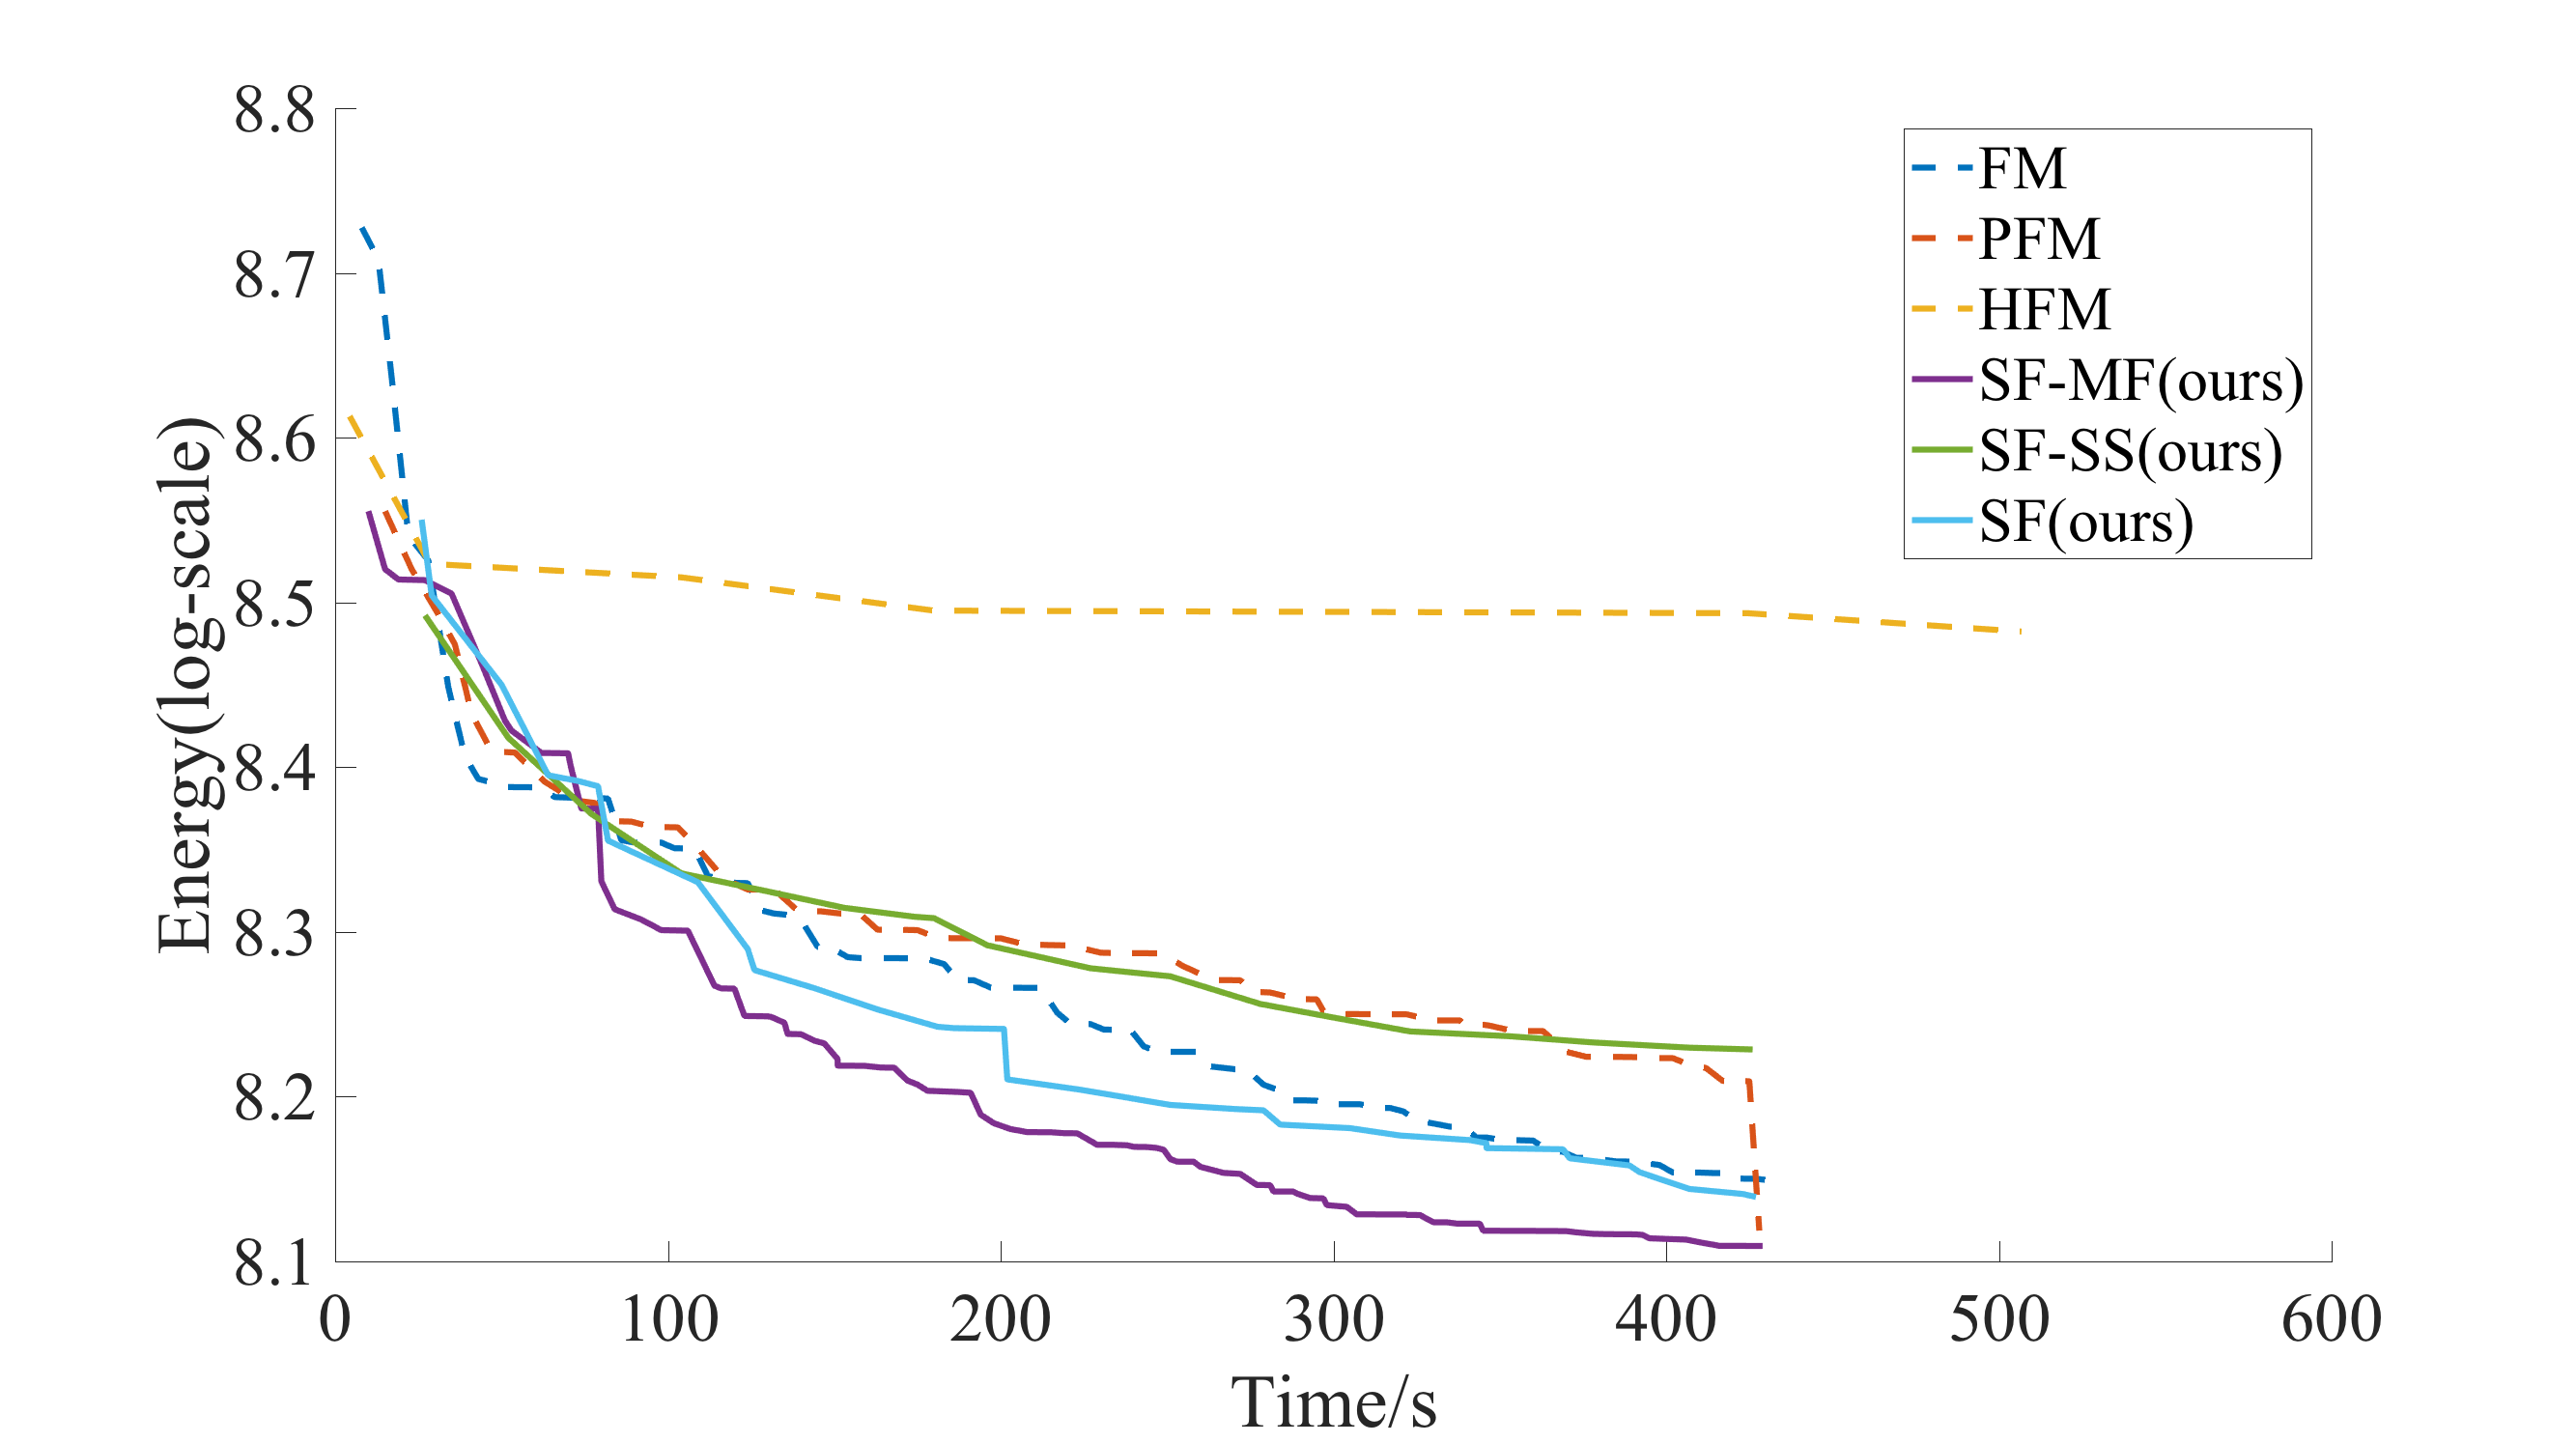
\includegraphics[width=\columnwidth]{figure/optical_flow_convergence.png}
  \caption{The energy minimization process for optical flow estimation of different methods. FS-MF has the best performance because of the solution sharing in early stage.}\label{fig:optical_flow_convergence}
\end{figure}
\begin{figure}[tb]
  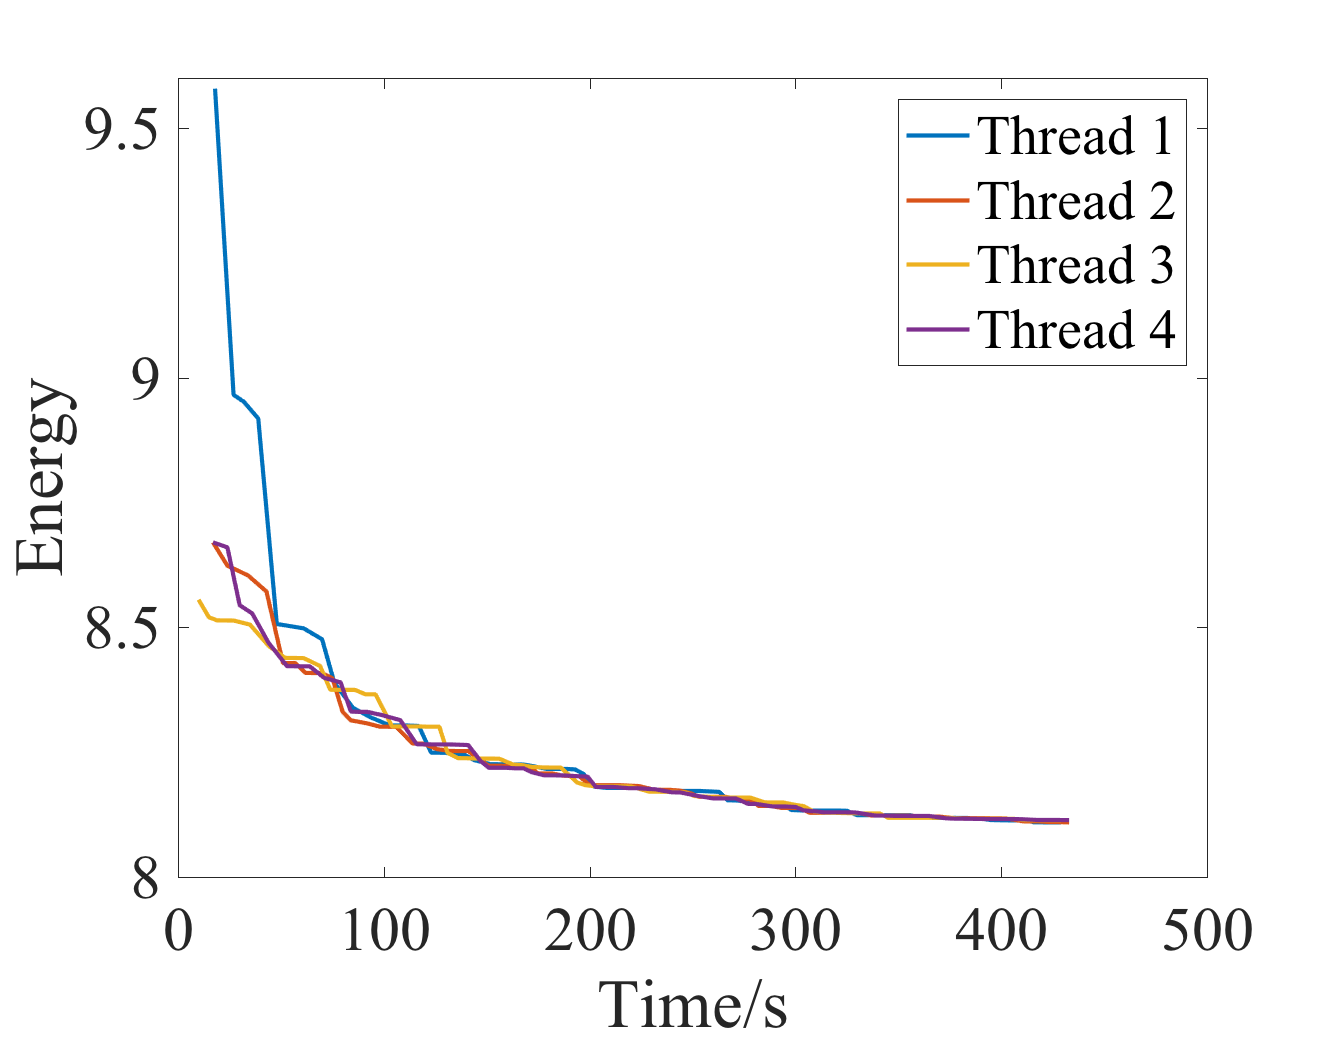
\includegraphics[width=0.5\columnwidth]{figure/optical_flow_SF_MF_threads.png}
  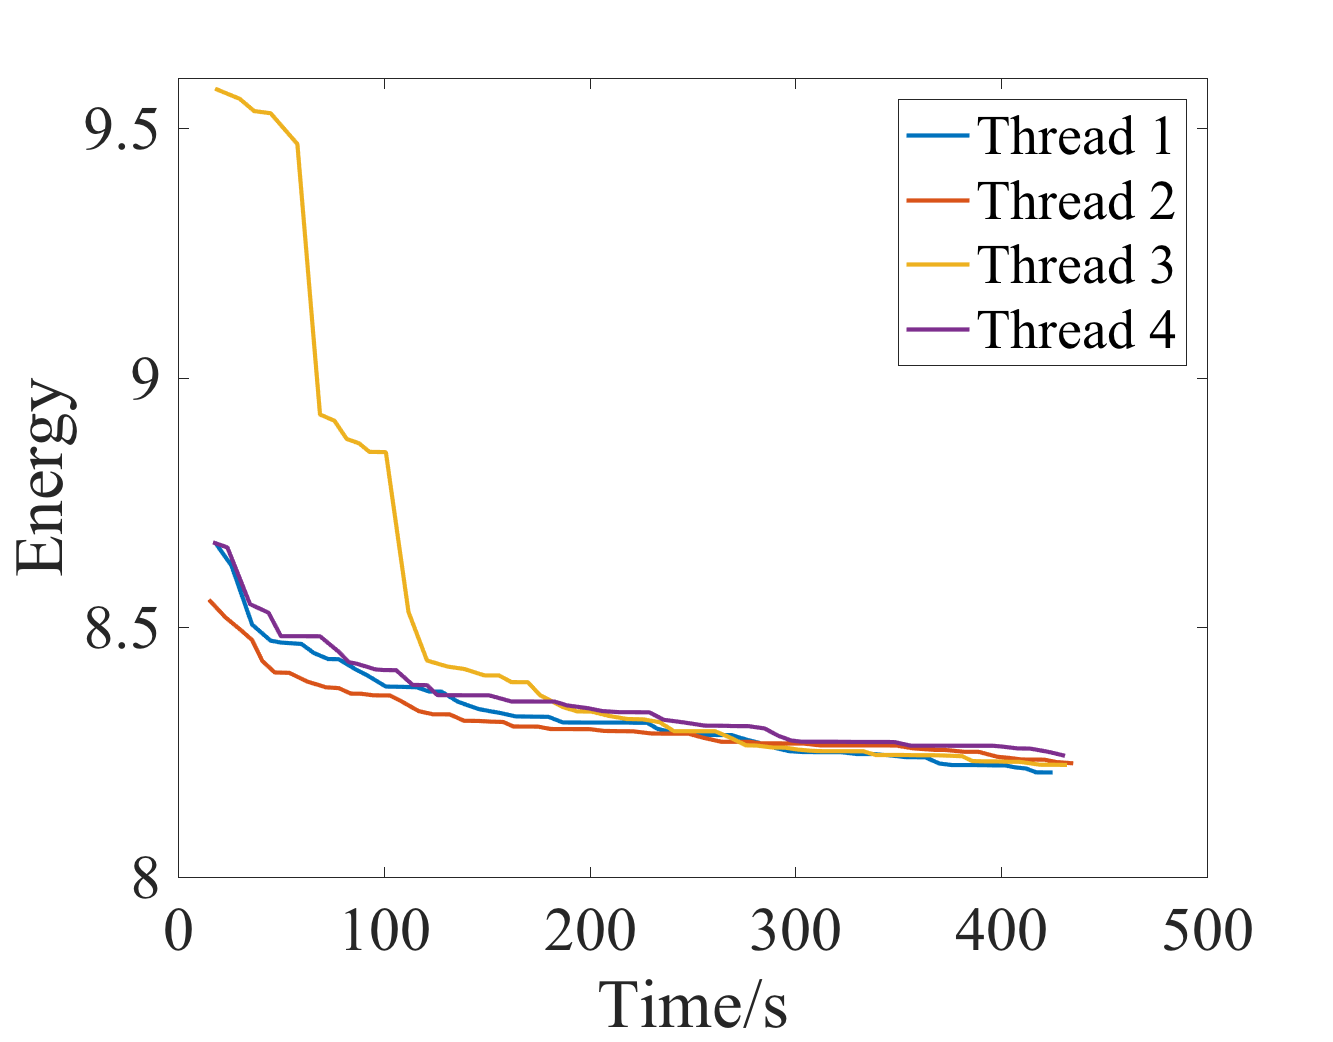
\includegraphics[width=0.5\columnwidth]{figure/optical_flow_PFM_threads.png}
  \caption{Per thread energy. The left and right figures show the energy minimization process on each working thread of our method in SF-MF configuration and parallel fusion move, respectively.}\label{fig:optical_flow_by_threads}
\end{figure}
\begin{figure}[tb]
  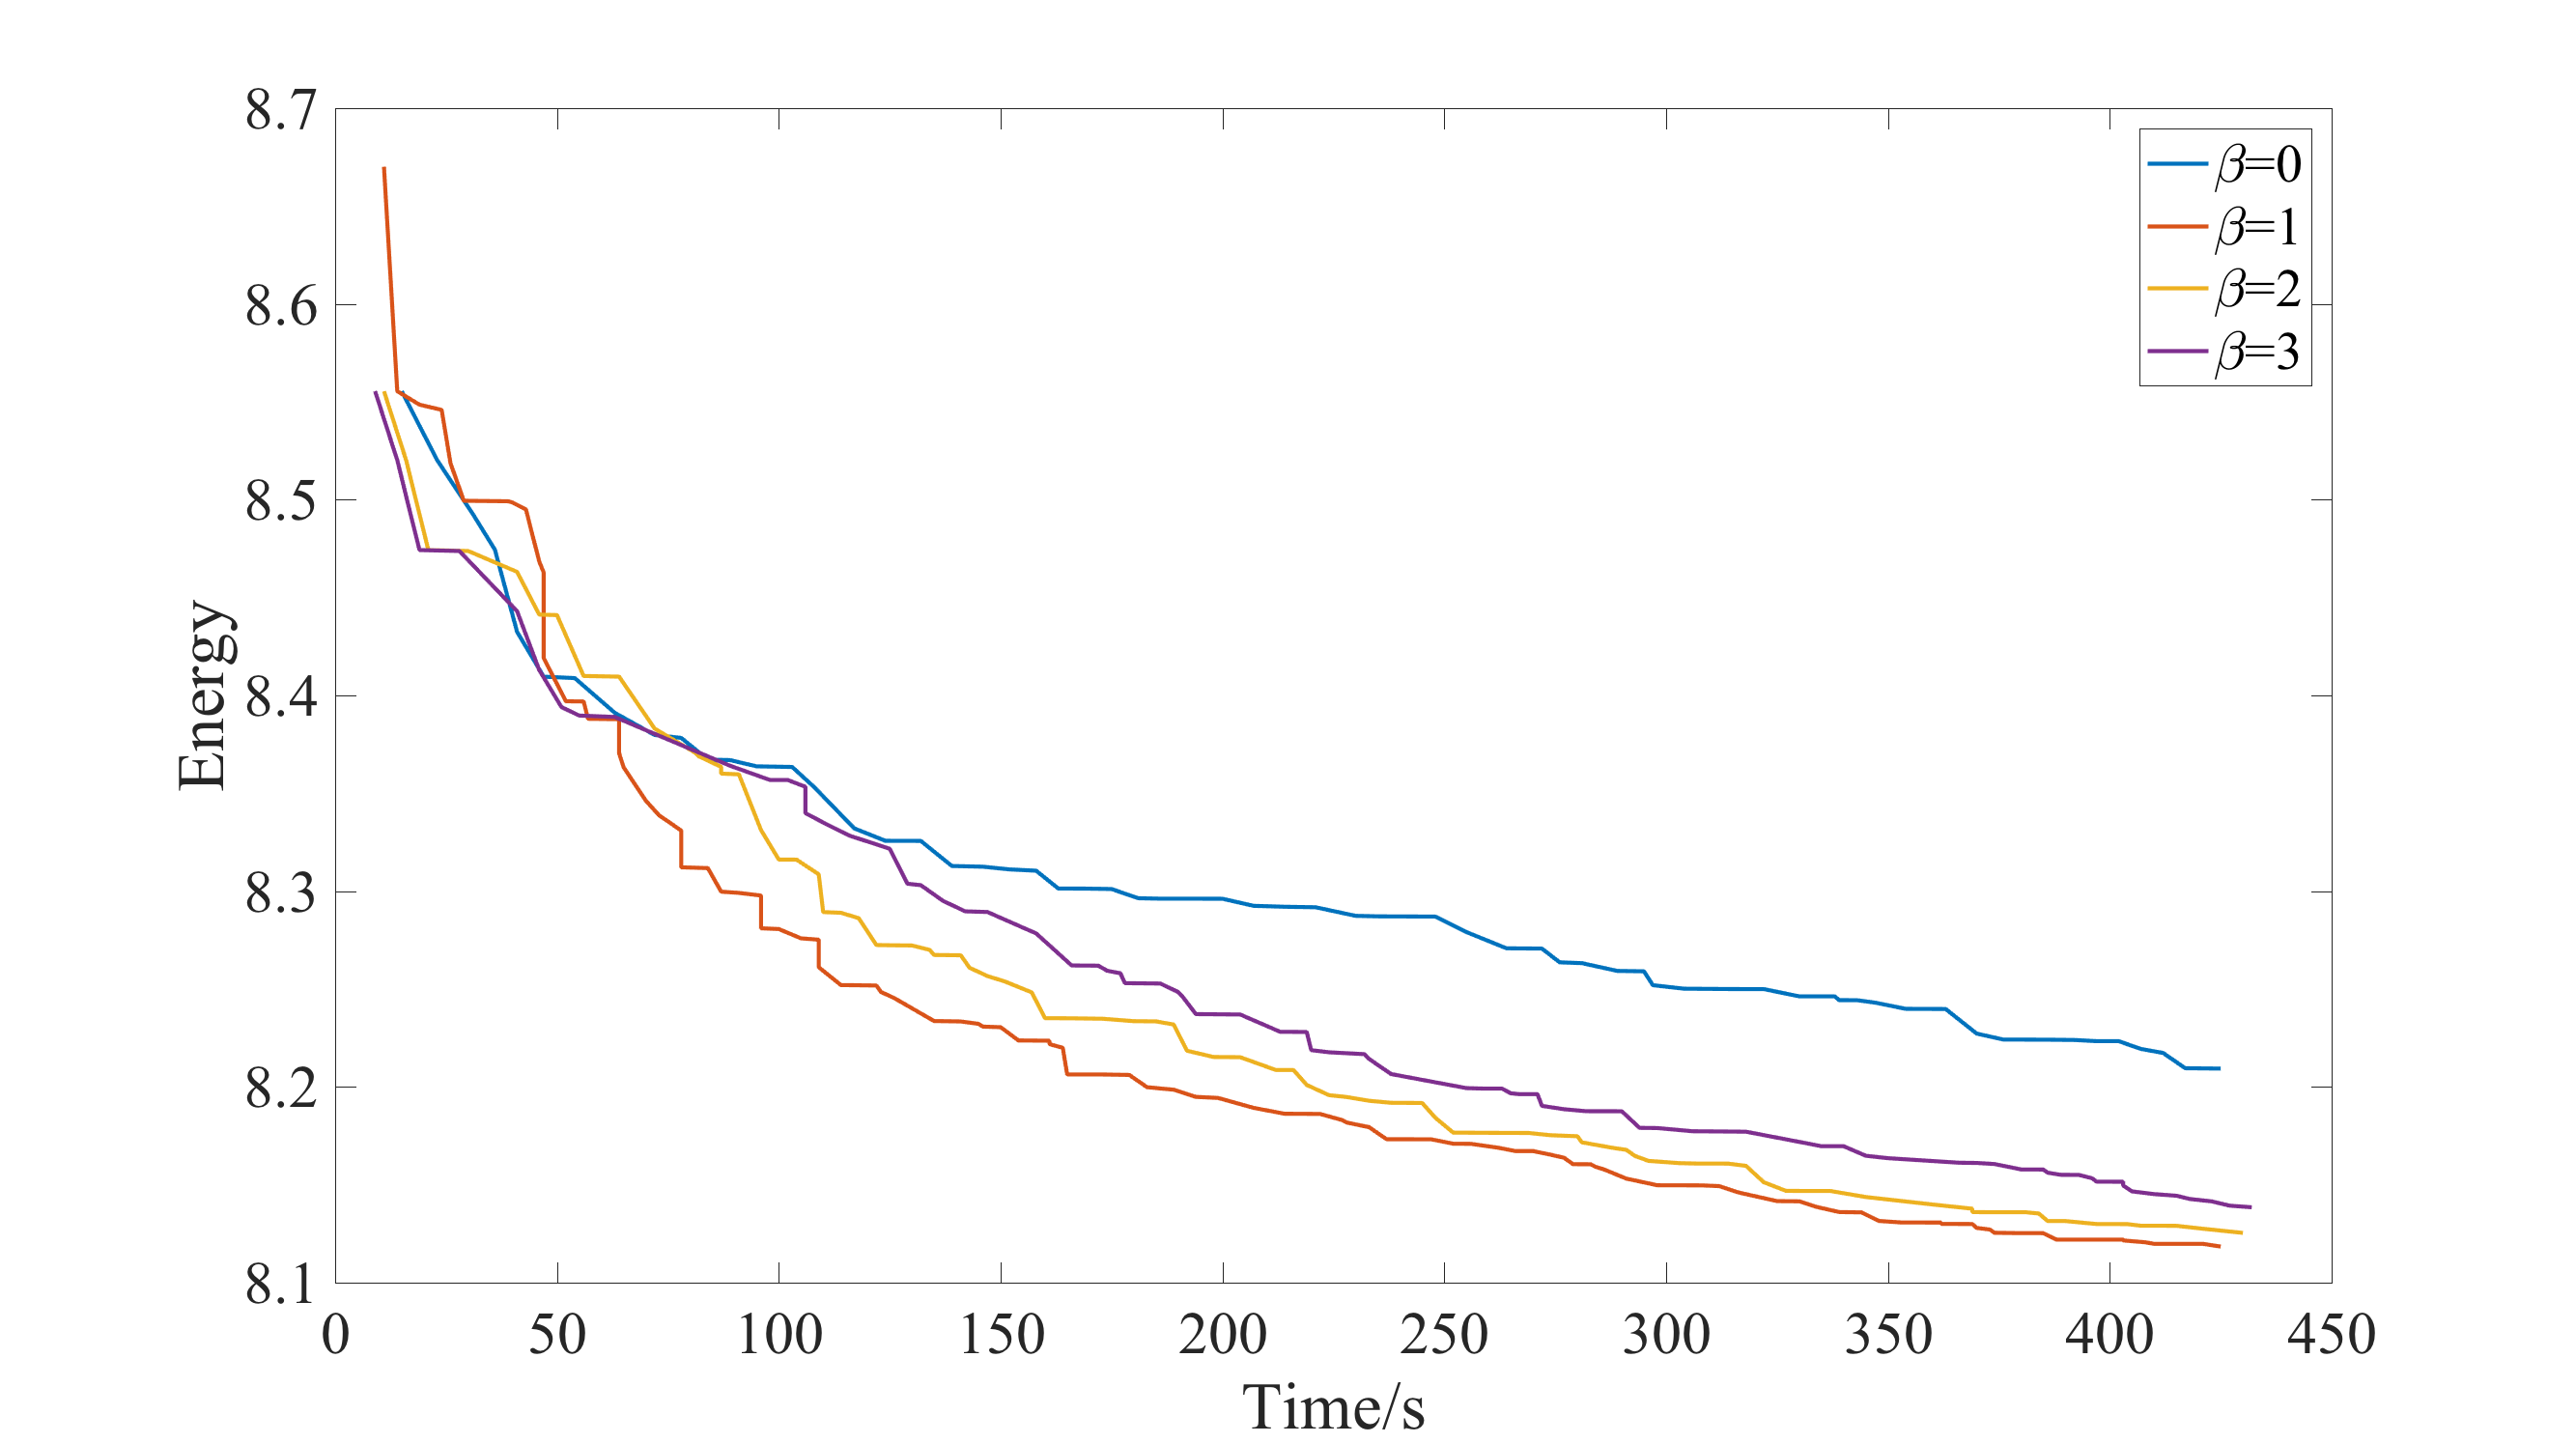
\includegraphics[width=\columnwidth]{figure/optical_flow_by_beta.png}
  \caption{The energy minimization process for optical flow estimation with different $\beta$ values. Solution sharing generally makes energy minimization faster, but more solution sharing also means less time for exploring new solution proposals.}\label{fig:optical_flow_by_beta}
\end{figure}
\begin{figure}[tb]
  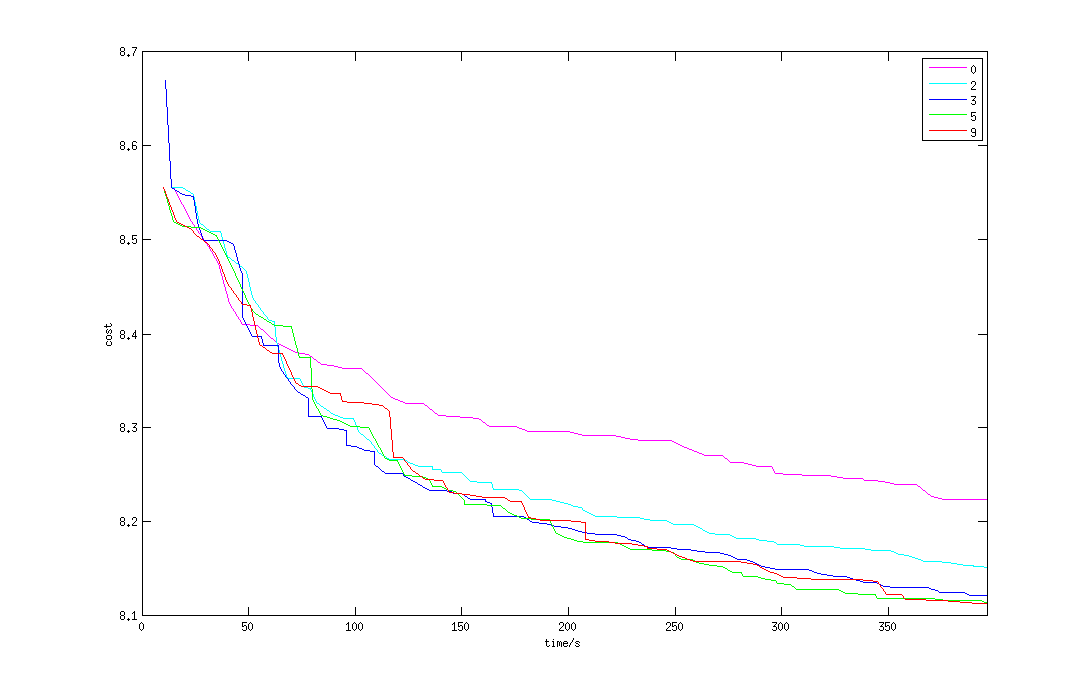
\includegraphics[width=\columnwidth]{figure/optical_flow_by_interval.png}
  \caption{The energy minimization process for optical flow estimation with different solution sharing frequency. Solution sharing generally makes energy minimization faster, but frequent solution sharing also means less time for exploring new solution proposals.}\label{fig:optical_flow_by_beta}\label{fig:optical_flow_by_interval}
\end{figure}

Figure \ref{fig:optical_flow_convergence} illustrates the convergence rate of three competing methods (alpha expansion, parallel alpha expansion, hierarchical fusion) against
our swarm fusion method. From the figure we can observe that, both conducting binary fusion, FS-MF finds lower energy faster than PFM. This is because some solution proposals are more effective than others, so once a thread grabs an effective solution proposal, it find a lower energy quickly. Since there is no solution sharing in PFM model, other threads cannot share this lower energy state, and keeps working on its own state. On the other hand, FS-MF allows solution sharing, so once a thread grabs an effective solution proposal and moves to a lower energy state, other threads can share this lower energy state. To further demonstrate what is happening here, we plot per thread energy in PFM and FS-MF in figure \ref{fig:optical_flow_by_threads}. As we can see from the plots, in PFM model, one thread finds lower energy state faster than others, while other threads keep working at their own energy state. But in FS-MF model, all threads exchange information about the lowest energy state and work on improving the lowest energy state together. So there are more chance of finding effective proposals faster. Since the solution for optical flow can be locally improved by each thread, the final merging of PFM can effectively fuse good local results in different threads together and achieve a similar energy state with FS-MF model. But since FS-MF model shares information in the middle, a final merging becomes less necessary. Same comparison holds for FS-SS and FS. The multi-way fusion is ineffective in this problem setting since solution proposals are relatively independant and fusing multiple solutions together using TRW-S~\cite{TRW-S} is less efficient than fusing them one by one using~\cite{QPBO}.

They are two factors influencing solution sharing: 1) \textit{the number of solutions to share} and 2) \textit{the solution sharing frequency}. Both factors are controlled by $\beta$. As mentioned in the section \label{optical_flow}, we use $\beta = 1$ once in every five iterations and use $\beta = 0$ for all other iterations. This means we share one solution in every five iterations. To further understand the effect of solution sharing, we did two other experiments for comparison. In one experiment, we use $\beta = {0, 1, 2, 3}$ in every five iterations and $\beta = 0$ for other iterations (when $\beta = 0$, it is same with PFM without final merging). While keeping all other factor same, we plot the energy minimization process in figure \ref{fig:optical_flow_by_beta}. As shown in the figure, energy generally decreases faster with solution sharing. But since we need to perform one fusion for sharing each solution, sharing more solution decreases efficiency in this problem setting. While sharing multiple solutions might be useful in some other problem setting as it means each thread can get more global information early. In another experiment, we change the number of iterations between two consecutive solution sharing iterations (the number of zero $\beta$ between two non-zero $\beta$) and plot the energy minimization process in figure \ref{fig:optical_flow_by_interval}. From this figure, we can see that although solution sharing generally speeds up the optimization process, sharing solution too frequently is not a good practice. This is because when we share solution frequently, we have less time for generating and fusing new proposals. A good choice of the solution sharing frequency depends on specific problem setting.

\mysubsubsection{Layered Depthmap}

\begin{figure}[tb]
  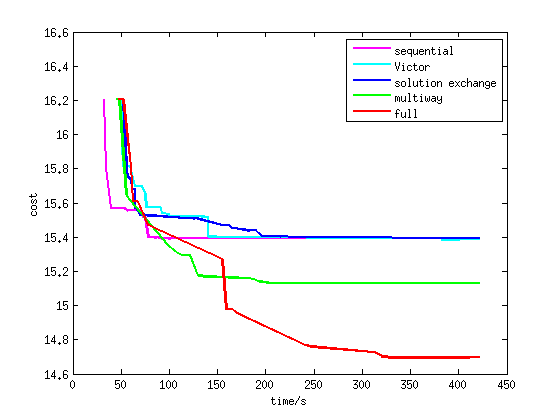
\includegraphics[width=\columnwidth]{figure/layered_depthmap_convergence.png}
  \caption{The energy minimization process for layered depthmap estimation of different methods. Multi-way fusion is shown to be more effectvie than binary fusion in this problem setting.}\label{fig:layered_depthmap_convergence}
\end{figure}
\begin{figure}[tb]
  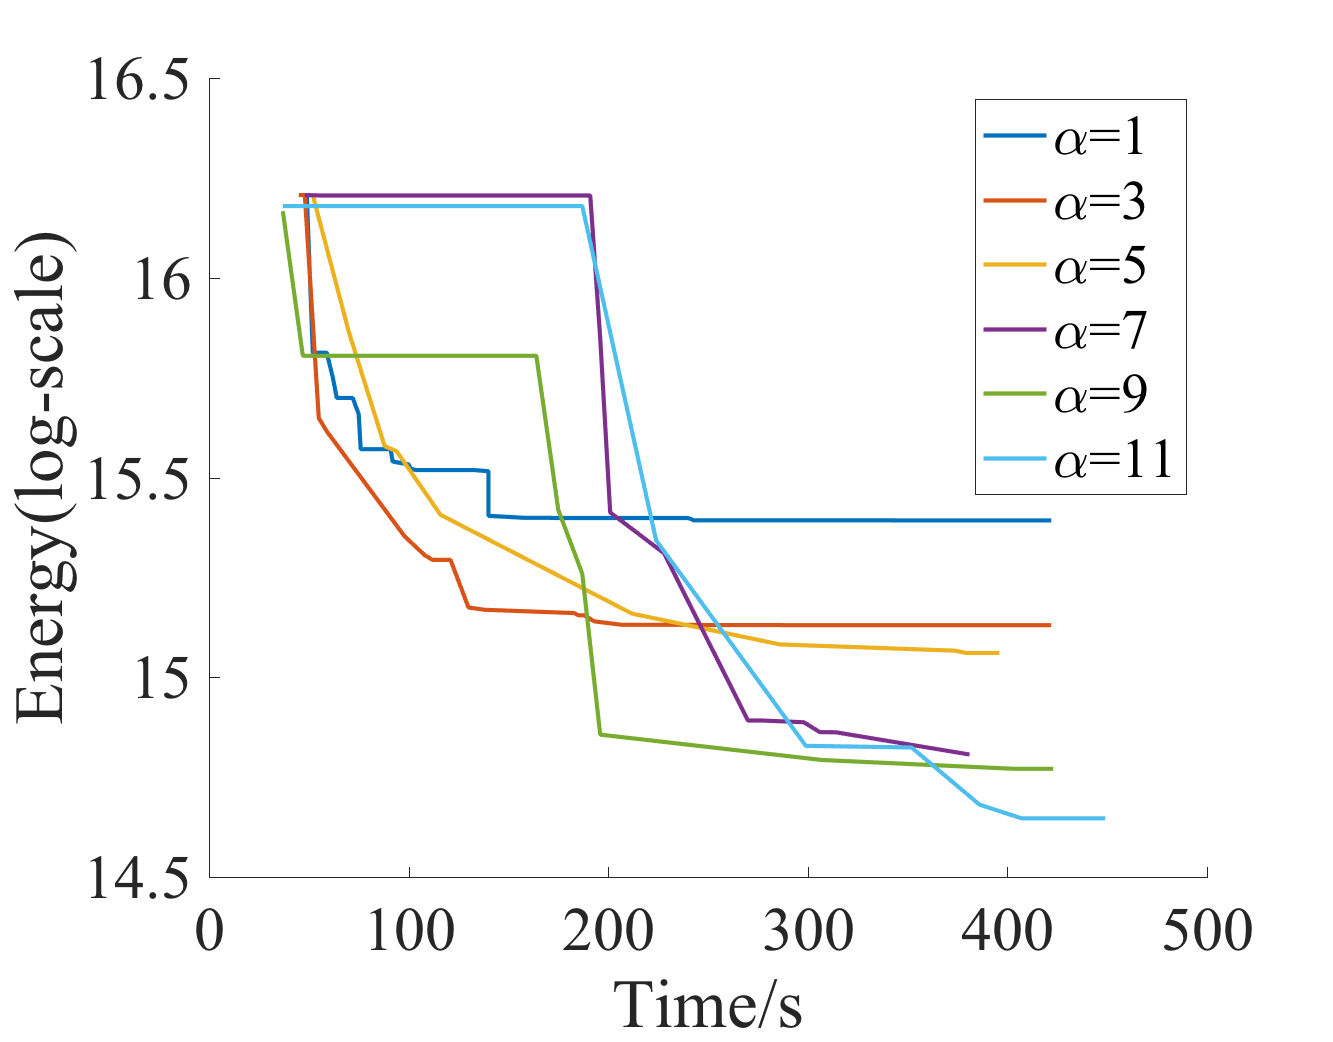
\includegraphics[width=\columnwidth]{figure/layered_depthmap_by_alpha.png}
  \caption{The energy minimization process for layered depthmap estimation with different $\alpha$ values. Multi-way fusion generally performs better than binary fusion, but the optimization becomes harder for using more ways in each step.}\label{fig:layered_depthmap_by_alpha}
\end{figure}

From the convergence plot of layered depth map estimation, we can see that, Fusion Move, Parallel Fusion Move, and FS-MF all stalk at a high energy state. The reason is binary fusion of solution proposals (either from others or self) is too limited to further decrease the energy due to the complexity of the problem itself. Only when multi-way fusion is used (in FS-SS and FS), it becomes possible for the energy to further decrease. This coincides with the observation in \cite{layered_depthmap} that binary fusion of proposal solutions is not as powerful as their subspace fusion which is a special form of multi-way fusion here. To further explore the effect of multi-way fusion, we use different $\alpha$ {1, 3, 7, 15} in FS model while keeping other parameters the same and plot the energy-time curve in figure \ref{fig:layered_depth_map_by_alpha}.

As shown in \ref{section:results}, the multi-way fusion and solution sharing enabled by our uniform framework play a key role for improving performance in different settings. For better understanding our framework, we examine the role played by each factor more closely by varying each factor while keeping others the same.




%As shown in the above problem settings, the solution sharing and
%multi-way fusion enabled by our uniform framework play a key role for
%improving performance in different problem settings.

